\chapter{Vergelykings en Ongelykhede}\fancyfoot[LO,RE]{Focus Area: Wiskunde}
\setcounter{figure}{1}
\setcounter{subfigure}{1}

\section{Oplos van lineêre vergelykings}
\nopagebreak
 $ \hspace{-5pt}\begin{array}{cccccccccccc}   
\includegraphics[width=0.75cm]{col11306.imgs/summary_fullmarks.png} &   
\includegraphics[width=0.75cm]{col11306.imgs/summary_video.png} &   \end{array} $ \hspace{2 pt}\raisebox{-5 pt}{} {(section shortcode: MG10068 )} \par 
           
Die eenvoudigste vergelyking om op te los is ’n lineêre vergelyking. ‘n Vergelyking word lineêr genoem indien
die hoogste mag van die veranderlike $1$ is. Die volgende is voorbeelde van lineêre
vergelykings:\par 


\begin{equation*}
\begin{array}{ccl}\hfill 2x+2& =& 1\hfill \vspace{6pt} \\
 \hfill \dfrac{2-x}{3x+1}& =& 2\hfill \vspace{6pt} \\
\hfill 4(2x-9)-4x&=&4-6x \hfill  \vspace{6pt}\\ 
\hfill \dfrac{2a-3}{3}-3a&=&\dfrac{a}{3} \hfill\\
\end{array}
\end{equation*}
In hierdie afdeling sal ons leer om te bepaal wat die waarde van ’n veranderlike moet wees om ’n vergelyking waar
te maak. Byvoorbeeld, watter waarde van $x$ maak beide kante van die baie eenvoudige vergelyking $x+1=1$ waar. Die oplossing is $x=0$.\par 
Aangesien die definisie van ’n lineêre vergelyking is dat die hoogste mag van die veranderlike een ($1$) moet wees,
is daar hoogstens een oplossing of wortel vir die vergelyking.\par 
Hierdie afdeling berus op al die metodes wat ons reeds bespreek het: uitvermenigvuldiging van uitdrukkings met
hakies, groepering van terme en faktorisering.\par 

\begin{equation*}
  \begin{array}{ccll}\hfill 2x+2& =& 1\hfill \\ 
      \hfill 2x& =& 1-2\hfill & \mbox{(groepeer soortgelyke terme saam)}\hfill \\ 
      \hfill 2x& =& -1\hfill & \mbox{(vereenvoudig)}\hfill \\
\hfill x&=& -\frac{1}{2} & \mbox{(deel weerskante met $2$)} \hfill
  \end{array}
\end{equation*}

\begin{equation*}

\end{equation*}
Vervang  $x=-\frac{1}{2}$ in die oorspronklike vergelyking. Dan kry ons:

\begin{equation*}
    \begin{array}{ccl}\hfill \mbox{LK}& =& 2x+2\hfill \\
	  & =& 2(-\frac{1}{2})+2\hfill \\
	  & =& -1+2\hfill \\
	  & =& 1\hfill \\
	  \hfill \mbox{RK}& =& 1\hfill \\
    \end{array}
\end{equation*}
Daarom is $x = -\frac{1}{2}$ 'n geldige oplossing

\Tip{Wanneer jy die oplossing van ’n vergelyking gevind het, vervang die oplossing
in die oorspronklike vergelyking om jou antwoord te bevestig.}

\subsection*{Metode: Oplos van lineêre vergelykings}

Die algemene stappe in die oplos van lineêre vergelykings is:
\begin{enumerate}[noitemsep, label=\textbf{\arabic*}. ] 
    \item Verwyder alle hakies in die vergelyking.
    \item Herrangskik die terme van die vergelyking sodat al die terme wat die veranderlike bevat aan een kant van die gelykaanteken is en alle konstantes aan die ander kant.
    \item Groepeer alle soortgelyke terme saam en vereenvoudig so ver as moontlik.
\item Faktoriseer, indien nodig.
    \item Vind die oplossing en skryf die antwoord(e) neer.
    \item Stel die oplossing in die oorspronklike vergelyking in om die antwoord te bevestig.
\end{enumerate}

\Tip{die twee kante van 'n vergelyking moet altyd balanseer; wat jy doen aan die een kant moet jy doen aan die ander kant. 'n moontlike oplossing van NIE de vergelyking bevredig nie, is nie geldig nie.}

\setcounter{subfigure}{0}
\begin{figure}[H] % horizontal\label{m39241*equations-1}
\textnormal{Khan academy video on equations - 1}\vspace{.1in} \nopagebreak
\label{m39241*yt-media1}\label{m39241*yt-video1}
\raisebox{-5 pt}{ 
\includegraphics[width=0.5cm]{col11306.imgs/summary_www.png}} { (Video:  MG10069 )}
\vspace{2pt}   $\theta $
    &

\vspace{.1in}
\end{figure}       

    
\begin{wex}{Oplos van lineêre vergelykings}
{
Los op vir $x$: $15-2x=3$
}
{
\westep{Herrangskik}

\begin{equation*}
    \begin{array}{cclc}\hfill 15-2x& =& 3\hfill & \\
	    \hfill -2x& =& 3-15\hfill & \hfill 
	    
    \end{array}
\end{equation*}

\westep{Vereenvoudig}
\begin{equation*}
    \begin{array}{cccc}\hfill -2x& =&-12\hfill & 
	    
    \end{array}
\end{equation*}

\westep{Deel weerskante met $-2$}
\begin{equation*}
    \begin{array}{cccc}\hfill x& =&6\hfill & 
	    
    \end{array}
\end{equation*}
\westep{Stel die oplossing in die oorspronklike vergelyking in om die antwoord te bevestig.}  

\begin{equation*}
\begin{array}{ccc}\hfill 15 - 2(6)& =& 3\hfill \\
 \hfill 15-12& =& 3\hfill \\
\hfill 3 &=& 3\hfill
\end{array}
\end{equation*}
Aangesien beide kante gelyk is, is die antwoord korrek
}
\end{wex}

\begin{wex}
{Los line\^ere vergelykings op }
{Los op vir $x$: $4(2x-9)-4x=4-6x$}
{
\westep{Brei die hakies uit en vereenvoudig}

\begin{equation*}
    \begin{array}{ccl}\hfill 4(2x-9)-4x& =& 4-6x\hfill  \\ 
	\hfill 8x-36-4x& =& 4-6x\hfill   \\ 
	\hfill 8x-4x+6x& =& 4+36\hfill  \\ 
	\hfill (8x-4x+6x)& =& (4+36)\hfill   \\   
	\hfill 10x& =& 40\hfill  
    \end{array}
\end{equation*}

\westep{Deel weerskante deur $10$}
\begin{equation*}
    \begin{array}{ccl}
	\hfill \dfrac{10}{10}x& =& \dfrac{40}{10}\hfill\\
	\hfill x& =& 4\hfill  
    \end{array}
\end{equation*}

\westep{Stel die oplossing in die oorspronklike vergelyking in}  

\begin{equation*}
    \begin{array}{ccl}\hfill 4[2(4)-9]-4(4)& =& 4-6(4)\hfill \\
	\hfill 4(8-9)-16& =& 4-24\hfill \\
	\hfill 4(-1)-16& =& -20\hfill \\
	\hfill -4-16& =& -20\hfill \\
	\hfill -20& =& -20\hfill 
    \end{array}
\end{equation*}
Aangesien beide kante gelyk is, is die antwoord korrek 
}
\end{wex}

\begin{wex}{Oplos van lineêre vergelykings}
{Los op vir $x$: $\dfrac{2-x}{3x+1}=2$} 
{
\westep{Ons begin deur weerskante van die vergelyking te vermenigvuldig met $(3x+1)$}
Omdat deling met $0$ ontoelaatbaar is, is daar ’n beperking op die waarde van ($x\neq -\frac{1}{3}$)

\begin{equation*}
    \begin{array}{ccll}\hfill \dfrac{2-x}{3x+1}& =& 2\hfill & \\
	\hfill (2-x)& =& 2(3x+1)\hfill & \\ 
    \end{array}
\end{equation*}

\westep{Brei hakies uit en vereenvoudig}
\begin{equation*}
    \begin{array}{ccll}
	\hfill 2-x& =& 6x+2\hfill & \hfill \\ 
	\hfill -x-6x& =& 2-2\hfill & \hfill \\ 
	\hfill -7x& =& 0\hfill & \hfill
    \end{array}
\end{equation*}

\westep{Deel weerskante deur $-7$}
\begin{equation*}
    \begin{array}{ccll}

	\hfill x& =& \dfrac{0}{-7}\hfill & \\
	\hfill x& =& 0\hfill & \hfill 
    \end{array}
\end{equation*}
Let op dat $0$ gedeel deur enige ander getal is $0$.

\westep{Stel die oplossing in die oorspronklike vergelyking in:}

\begin{equation*}
    \begin{array}{ccc}\hfill \dfrac{2-(0)}{3(0)+1}& =& 2\hfill \vspace{6pt}\\
	\hfill 2& =& 2\hfill 
\end{array}
\end{equation*}
Aangesien weerskante gelyk is, is die antwoord korrek
}
\end{wex}


\begin{wex}
{Oplos van lineêre vergelykings}
{Los op vir $a$: $\dfrac{2a-3}{3}-3a=\dfrac{a}{3}$}
{
\westep{Ons begin deur elk van die terme in die vergelyking te vermenigvuldig met  $3$ en vervolgens te vereenvoudig.}  

\begin{equation*}
    \begin{array}{cccc}\hfill 2a-3 - 9a &= &a\hfill & \\ 
\hfill -7a - 3 &= &a\hfill & 
    \end{array}
\end{equation*}

\westep{Herrangskik en vereenvoudig}
\begin{equation*}
    \begin{array}{cccc}\hfill -7a -a &= &3\hfill & \\ 
\hfill -8a &= &3\hfill & \\
    \end{array}
\end{equation*}

\westep{Deel weerskante deur $-8$} 
\begin{equation*}
    \begin{array}{cccc}\hfill a &= & -\dfrac{3}{8}\hfill & \\ 

    \end{array}
\end{equation*}

\westep{Stel die oplossing in die oorspronklike vergelyking in:}
\begin{equation*}
    \begin{array}{ccll}\hfill \dfrac{2(-\frac{3}{8}) - 3}{3} - 3(-\frac{3}{8}) &= & \dfrac{-\frac{3}{8}}{3}\hfill & \\ 
\\
      \hfill \dfrac{(-\frac{3}{4}) - \frac{12}{4}}{3} + \frac{9}{8} &= & \dfrac{-\frac{3}{8}}{3}\hfill & \\ 
\\
 \hfill \Bigg[-\frac{15}{4} \times \frac{1}{3}\Bigg] + \frac{9}{8} &= & -\frac{3}{8} \times \frac{1}{3}\hfill & \\ 
\\
 \hfill -\frac{5}{4} + \frac{9}{8} &= & -\frac{1}{8}\hfill & \\ 
 \hfill -\frac{10}{8} + \frac{9}{8} &= & -\frac{1}{8}\hfill & \\ 
 \hfill -\frac{1}{8} &= & -\frac{1}{8}\hfill & 
    \end{array}
\end{equation*}
Beide kante is gelyk, dus die oplossing is reg.
}
\end{wex}

\begin{exercises}{}
{
Oplos van lineêre vergelykings: \\
Aanvaar alle noemers is non-zero.
\begin{multicols}{2}
\begin{enumerate}[noitemsep, label=\textbf{\arabic*}. ] 
\item   $2y-3=7$
\item   $-3y=0$        
\item   $16y+4=-10$        
\item   $12y+0=144$
\item   $7+5y=62$   \vspace{6pt}     
\item  $55=5x+\dfrac{3}{4}$ \vspace{6pt}
\item   $5x=2x+45$        
\item  $23x-12=6+3x$
\item   $12-6x+34x=2x-24-64$
\item   $6x+3x=4-5(2x-3)$
\item   $18-2p=p+9$   \vspace{6pt}
\item   $\dfrac{4}{p}=\dfrac{16}{24}$
\item   $-(-16-p)=13p-1$
\item   $3f-10=10$
\item   $3f+16=4f-10$
\item   $10f+5=-2f-3f+80$
\item   $8(f-4)=5(f-4)$
\item  $6=6(f+7)+5f$      
\item $(a-1)^{2} - 2a = (a+3)(a-2) - 3$
\item $-7x = x+8(1-x)$ \vspace{6pt}
\item $5-\dfrac{7}{b} = \dfrac{2(b+4)}{b}$\vspace{6pt}
\item $\dfrac{x+2}{4} - \dfrac{x-6}{3} = \dfrac{1}{2}$\vspace{6pt}
\item $ 3 - \dfrac{y-2}{4} = 4$\vspace{6pt}
\item $ \dfrac{a+1}{a+2} = \dfrac{a-3}{a+1}$
  
\end{enumerate}
\end{multicols}
\par \raisebox{-5 pt}{
\includegraphics[width=0.5cm]{col11306.imgs/summary_www.png}} Kry die oplossing met die kortkodes:
\par \begin{tabular}[h]{cccccc}
(1.) lcR  &  (2.) lcR  &  (3.) lcR  &  (4.) lcR  &  (5.) lcR  &  (6.) lcn  &  (7.) lcn  &  (8.) lcn  &  (9.) lcn  &  (10.) lcn  &  (11.) lcQ  &  (12.) lcQ  &  (13.) lcQ  &  (14.) lcQ  &  (15.) lcQ  &  (16.) lcU  &  (17.) lcU  &  (18.) lcU  &  (19.) lcU  &  (20.) lcU  & \end{tabular}
}
\end{exercises}

\section{Oplos van kwadratiese vergelykings}

 $ \hspace{-5pt}\begin{array}{cccccccccccc}   
\includegraphics[width=0.75cm]{col11306.imgs/summary_fullmarks.png} &   
\includegraphics[width=0.75cm]{col11306.imgs/summary_video.png} &   \end{array} $ \hspace{2 pt}\raisebox{-5 pt}{} {(section shortcode: MG10070 )}       \par
’n Kwadratiese vergelyking, is ’n vergelyking waar die mag van die veranderlike hoogstens
$2$ is. \\Die volgende is voorbeelde van kwadratiese vergelykings:\par 


\begin{equation*}
    \begin{array}{ccl}\hfill 2{x}^{2}+2x& =& 1\hfill \\
	\hfill 3{x}^{2}+2x-1&=&0 \\ 
	\hfill 0&=&-2{x}^{2}+4x-2\hfill 
    \end{array}
\end{equation*}

Kwadratiese vergelykings verskil van lineêre vergelykings daarin dat ’n lineêre vergelyking slegs een oplossing
het, terwyl ‘n kwadratiese vergelyking hoogstens 2 oplossings het. Daar is spesiale gevalle waar ’n kwadratiese
vergelyking slegs een oplossing het.

\begin{aktiwiteit}{}
Los die Kwadratiese Vergelykings $x^{2}=16$ op deur drie verskillende metodes te gebruik:
\begin{enumerate}[noitemsep, label=\textbf{\arabic*}. ] 
\item Inspeksie (probeer en toets)
\item Trek die vierkantswortels
\item Faktorisering
\end{enumerate}
(Let op, indien $a \times b = 0$ dan $a = 0$ of $b=0$)
\end{activity}

Ons kan 'n kwadratiese vergelyking oplos deur faktorisering te gebruik. Byvoorbeeld, om $2{x}^{2}-x-3 = 0$ op te los, moet ons die uitdrukking in sy ekwivalente gefaktoriseerde vorm skryf as $(x+1)(2x-3)=0$.


\subsection*{Metode: Oplos van kwadratiese vergelykings}
\begin{enumerate}[noitemsep, label=\textbf{\arabic*}. ] 
\item Skryf die vergelyking die vorm $ax^{2} +bx +c =0$.
\item Deel heel eerste die hele vergelyking deur enige gemene faktore van die koëffisiënte, ten einde ’n vergelyking te kry van die vorm $a{x}^{2}+bx+c=0$ waar $a$, $b$ en
$c$ geen gemeenskaplike faktore het nie. Byvoorbeeld $2{x}^{2}+4x+2=0$ kan geskryf word as
${x}^{2}+2x+1=0$ deur te deel met $2$.
\item Skryf $a{x}^{2}+bx+c=0$ in terme van sy faktore  $(rx+s)(ux+v)=0$.

\item $(rx+s)=0$ of $(ux+v)=0$, so die oplossing is $x = -\dfrac{s}{r}$ of $x=-\dfrac{v}{u}$.
\item Vervang elke moontlike waarde van die oplossing in die oorspronklike vergelyking in om te toets of dit ’n
geldige oplossing is.

\end{enumerate}

% \label{m39247*eip-388}
\setcounter{subfigure}{0}
\begin{figure}[H] % horizontal\label{m39247*equations-3}
\textnormal{Khan academy video on equations - 3}\vspace{.1in} \nSolve 
\label{m39247*yt-media3}\label{m39247*yt-video3}
\raisebox{-5 pt}{ 
\includegraphics[width=0.5cm]{col11306.imgs/summary_www.png}} { (Video:  MG10071 )}
\vspace{2pt}
\vspace{.1in}
\end{figure}

        
\begin{wex}
{Oplos van kwadratiese vergelykings }
{Los op vir $x$: $3{x}^{2}+2x-1=0$}
{
\westep{Die vergelyking in die regte vorm ${ax}^{2} + bx + c = 0$}

\westep{Faktoriseer}
\begin{equation*}
(x+1)(3x-1)=0
\end{equation*}

\westep{Los op vir beide wortels}
Ons het
\begin{equation*}
     \begin{array}{ccc}\hfill x+1&=&0\hfill \\
	\hfill \therefore x&=&-1
    \end{array}
\end{equation*}

of
\begin{equation*}
     \begin{array}{ccc}\hfill 3x-1&=&0\hfill \\
	\hfill \therefore x&=&\frac{1}{3}
    \end{array}
\end{equation*}
\westep{Kontroleer beide antwoorde deur instelling in die oorspronklike vergelyking.}
\westep{Skryf die finale antwoord}
Die oplossing van $3{x}^{2}+2x-1=0$ is dus $x=-1$ of $x=\frac{1}{3}$.
}
\end{wex}


\begin{wex}{ Oplos van kwadratiese vergelykings }
{ Vind die wortels van die kwadratiese vergelyking  $0=-2{x}^{2}+4x-2$}
{
\westep{Deel weerskante van die vergelyking deur $-2$}

\begin{equation*}
\begin{array}{ccc}\hfill -2{x}^{2}+4x-2& =& 0\hfill \\ \hfill {x}^{2}-2x+1& =& 0\hfill \end{array}
\end{equation*}

\westep{Die vergelyking is in die regte vorm ${ax}^{2} + bx + c = 0$}

\westep{Faktoriseer}
\begin{equation*}
\begin{array}{ccc} \hfill (x-1)(x-1) &=& 0 \hfill \\
\hfill (x-1)^{2} &=&0 \hfill 
\end{array}
\end{equation*}

\westep{ Die kwadratiese uitdrukking is ’n volkome vierkant}
Hierdie is a voorbeeld van 'n spesiale situasie waar daar net een oplossing vir die Kwadratiese Vergelykings is
\begin{equation*}
\begin{array}{ccc} \hfill x -1 &=& 0 \hfill \\
\hfill \therefore x &=&1 \hfill 
\end{array}
\end{equation*}

\westep{Stel die oplossing in die oorspronklike vergelyking in om dit te toets.}

 
\westep{Skryf die finale antwoord}
Die oplossing van $0=-2{x}^{2}+4x-2$ is $x=1$.
}
\end{wex}


\begin{exercises}{ }
{
Oplos van kwadratiese vergelykings:
\begin{multicols}{2}
\begin{enumerate}[noitemsep, label=\textbf{\arabic*}. ] 
\item  $(3x+2)(3x-4)=0$
\item  $(5x-9)(x+6)=0$
\item  $(2y+3)(2y-3)=0$ 
\item  $(2x+1)(2x-9)=0$    
\item  $(4x)(x-3)=-9$       
\item  $20m+25{m}^{2}=0$
\item  $2{x}^{2}-5x-12=0$  
\item  $-75{x}^{2}+290x=240$
\item  $2x=\frac{1}{3}{x}^{2}-3x+14\frac{2}{3}$
\item  ${x}^{2}-4x=-4$      
\item  $-{x}^{2}+4x-6=4{x}^{2}-5x+3$       
\item  ${t}^{2}=3t$  
\item  ${x}^{2}-10x=-25$      
\item  ${x}^{2}=18$
\item  ${p}^{2}-6p=7$
\item  $4{x}^{2}-17x-77=0$
\item  $14{x}^{2}+5x=6$
\item  $2{x}^{2}-2x=12$              
\end{enumerate}
\end{multicols}
\par \raisebox{-5 pt}{
\includegraphics[width=0.5cm]{col11306.imgs/summary_www.png}} Kry die oplossing met die kortkodes:
\par\begin{tabular}[h]{cccccc}
(1.) lcP  &  (2.) lcP  &  (3.) lcP  &  (4.) lcP  &  (5.) lcP  &  (6.) lcE  &  (7.) lcE  &  (8.) lcE  &  (9.) lcE  &  (10.) lcE  &  (11.) lcE  &  (12.) lcm  &  (13.) lcm  &  (14.) lcm  &  (15.) lcm  &  (16.) lcm  &  (17.) lcm  &  (18.) lcm  &  (19.) lcm  & \end{tabular}
}
\end{exercises}
% %          \section{ Exponential equations}
% %     \nopagebreak
% %             \label{m39253} $ \hspace{-5pt}\begin{array}{cccccccccccc}   
\includegraphics[width=0.75cm]{col11306.imgs/summary_fullmarks.png} &   \end{array} $ \hspace{2 pt}\raisebox{-5 pt}{} {(section shortcode: MG10072 )} \par 
% %     
% %     
\section{oplos van gelyktydige vergelykings}
$ \hspace{-5pt}\begin{array}{cccccccccccc}   
\includegraphics[width=0.75cm]{col11306.imgs/summary_fullmarks.png} &   
\includegraphics[width=0.75cm]{col11306.imgs/summary_video.png} &   \end{array} $ \hspace{2 pt}\raisebox{-5 pt}{} {(section shortcode: MG10076 )} \par

Tot dusver het alle vergelykings slegs een onbekende veranderlike gehad wat ons moes vind.
Wanneer twee onbekendes bepaal moet word, het ons twee vergelykings nodig. Hierdie vergelykings word gelyktydige vergelykings
genoem. Die oplossing vir die stelsel van gelyktydige vergelykings is die waardes van die veranderlikes wat die stelsel van vergelykings gelyktydig sal bevredig. In die algemeen beteken dit indien daar $n$ onbekende veranderlikes is, benodig ons $n$ vergelykings om ’n oplossing vir elk van die $n$ veranderlikes te vind.\par 
’n Voorbeeld van stel gelyktydige vergelykings is:

\begin{equation*}
\begin{array}{rcl} x+y&=&-1 \\ 
 3&=&y-2x 
\end{array}
\end{equation*}

Om ’n numeriese waarde vir onbekende veranderlikes te vind, moet ons ten minste soveel onafhanklike vergelykings as veranderlikes hê. Ons kan gelyktydige vergelykings algebraïes of grafies oplos.\par 
\setcounter{subfigure}{0}
\begin{figure}[H] % horizontal\label{m39257*simultaneous-equations}
\textnormal{Khan academy video on simultaneous equations - 1}\vspace{.1in} \nopagebreak
\label{m39257*yt-media7}\label{m39257*yt-video7}
\raisebox{-5 pt}{ 
\includegraphics[width=0.5cm]{col11306.imgs/summary_www.png}} { (Video:  MG10077 )}
\vspace{2pt}
\vspace{.1in}
\end{figure}       

\subsection*{Oplossing deur vervanging}
\begin{itemize}
 \item Probeer om een van die vergelykings op te los vir een van die veranderlikes.
\item Vervang die resultaat in die ander vergelykings. Deur dit te doen verminder die hoeveelheid
vergelykings en ook die hoeveelheid onbekende veranderlikes met 1.
\item Hierdie proses word herhaal tot ‘n enkele vergelyking met 1 veranderlike oorbly, wat (hopelik) opgelos kan word.
\item Vervang heirdie oplossing terug in die oorspronklike vergelyking om die waarde te vind van die ander onbekende veranderlike.
\end{itemize}

\Note{As die vraag nie spesifiek vra vir 'n grafiese oplossing nie, behoort die stelsel van gelyktydige vergelykings algebra\"ies opgelos te word.}

\begin{wex}
{Gelyktydige vergelykings}
{
Los die volgende stelsel gelyktydige vergelykings op:
\begin{equation*}
\begin{array}{ccl}\hfill x-y& =& 1\hfill \\ \hfill 3& =& y-2x\hfill \end{array}
\end{equation*}
}
{
\westep{los die eerste vergelyking op vir $x$ in terme van $y$}
\begin{equation*}
    \begin{array}{ccl}\hfill x& =& y+1\hfill 
    \end{array}
\end{equation*}

\westep{Stel hierdie resultaat in die tweede vergelyking in: $y$}
\begin{equation*}
    \begin{array}{ccl}\hfill 3& =& y-2(y+1)\hfill \\
	\hfill 3& =& y - 2y - 2\hfill \\
	\hfill 5& =& -y\hfill \\
\hfill \therefore y& =& -5\hfill
    \end{array}
\end{equation*}

\westep{Vervang nou terug in die oorspronklike vergelyking in en solvelos op vir $x$}
\begin{equation*}
    \begin{array}{ccl}\hfill x - (-5)& =& 1\hfill \\
	\hfill x+ 5& =& 1\hfill \\
\hfill \therefore x& =& -4\hfill
    \end{array}
\end{equation*}

\westep{Toets oplossing deur instelling in beide oorspronklike vergelykings}  

\westep{Skryf die finale antwoord}
\begin{equation*}
\begin{array}{ccl}\hfill y& =& -5\hfill \\
 \hfill x& =& -4\hfill 
\end{array}
\end{equation*}
}
\end{wex}

\begin{wex}
{Gelyktydige vergelykings}
{
Los die volgende stelsel gelyktydige vergelykings op:
\begin{equation*}
\begin{array}{ccc}\hfill 4y+3x& =& 100\hfill \\ 
\hfill 4y - 19x& =& 12\hfill 
\end{array}
\end{equation*}
}
{
\westep{Gebruik een van die vergelukings om $x$ uit te druk in terme van $y$}
\begin{equation*}
    \begin{array}{ccl}\hfill 4y+3x & =& 100\hfill \\
\hfill 3x &=& 100 - 4y \hfill \\
\hfill x& =& \dfrac{100 - 4y}{3} \hfill
    \end{array}
\end{equation*}


\westep{Vervan in die ander vergelyking om vir $y$ op te los}
\begin{equation*}
    \begin{array}{ccl}\hfill 4y - 19(\dfrac{100 - 4y}{3})& =& 12\hfill \\
	\hfill 12y - 19(100 - 4y)  & =& 36\hfill \\
	\hfill 12y - 1900 + 76y & =& 36 \hfill \\
\hfill  88y& =& 1936 \hfill \\
\hfill \therefore y& =& 22 \hfill
    \end{array}
\end{equation*}

\westep{Vervang terug in die eerste vergelyking en los op vir $x$}
\begin{equation*}
    \begin{array}{ccl}\hfill x &=& \dfrac{100 - 4(22)}{3}\hfill \vspace{6pt}\\
	\hfill & =& \dfrac{100-88}{3}\hfill \vspace{6pt}\\
	\hfill & =& \dfrac{12}{3}\hfill\vspace{6pt} \\
	\hfill \therefore x&=& 4 \hfill 
    \end{array}
\end{equation*}

\westep{Toets die oplossing deur instelling in beide oorspronklike vergelykings}  

\westep{Skryf die finale antwoord}
\begin{equation*}
\begin{array}{ccc}
 \hfill x& =& 4\hfill \\
\hfill y& =& 22\hfill 
\end{array}
\end{equation*}
}
\end{wex}

\subsection*{Los op deur eliminasie}

\begin{wex}
{Gelyktydige vergelukings}
{
Los die volgende stelsel van vergelykings op:
\begin{equation*}
\begin{array}{ccll}\hfill & 3x+y& =& 2\hfill \\ 

\hfill& 6x-y& =& 25\hfill 
\end{array}
\end{equation*}
}
{
\westep{Maak die ko\"effisi\"ente van een van die veranderlikes dieselfde in beide vergelykings}
Die ko\"effisie\"ente van $y$ is $1$ en $-1$. Elimineer die veranderlike $y$ deur die twee vergelykings bymekaar te tel
\begin{equation*}
\begin{array}{ccll}\hfill & 3x+y& =& 2\hfill \\ 
\hfill+ & 6x-y& =& 25\hfill \\ \hline
 \hfill & 9x + 0 &=& 27
\end{array}
\end{equation*}


\westep{Vereenvoudig en los op vir $x$}
\begin{equation*}
    \begin{array}{ccl}\hfill 9x& =& 27\hfill \\
	\hfill \therefore x  & =& 3\hfill 
    \end{array}
\end{equation*}

\westep{Vervang die waarde van $x$ terug in enige van die oorspronklike vergelykings en los op vir $y$}
\begin{equation*}
    \begin{array}{ccl}\hfill 3(3) + y &=& 2\\
	\hfill y & =& 2-9\\
	\hfill \therefore y & =& -7 
   \end{array}
\end{equation*}

\westep{Kontroleer dat die oplossing $x=3$ en $y=-7$ albei die oorspronklike vergelykings bevredig}  

\westep{Skryf die finale antwoord}
\begin{equation*}
\begin{array}{ccc}
 \hfill x& =& 3\hfill \\
\hfill y& =& -7\hfill 
\end{array}
\end{equation*}
}
\end{wex}

\begin{wex}
{Gelyktydige vergelykings}
{
Los die volgende stel gelyktydige vergelykings op:
\begin{equation*}
\begin{array}{cccc}\hfill & 2a - 3b& =& 5\hfill \\ 
\hfill& 3a-2b& =& 20\hfill 
\end{array}
\end{equation*}
}
{
\westep{Maak die ko\"effisi\"ente van enige van die veranderlikes dieselfde in beide vergelykings}
Vermenigvuldig die eerste vergelyking met $3$ en die tweede vergelyking met $2$, sodat beide ko\"effisi\"ente van $a$ $6$ sal wees.
\begin{equation*}
\begin{array}{cccc}\hfill & 6a-9b& =& 15\hfill \\ 
\hfill- & (6a-4b& =& 40)\hfill \\ \hline
 \hfill & 0 - 5b &=& -25 

\end{array}
\end{equation*}
(Wees versigtig met die teken as die een vergelyking van die ander afgetrek word.)

\westep{Vereenvoudig en los op vir $x$}
\begin{equation*}
    \begin{array}{ccl}
 \hfill b &=& \dfrac{-25}{-5} \\
 \hfill \therefore b &=& 5
    \end{array}
\end{equation*}

\westep{Vervang die waarde van $b$ terug in enige van die oorspronklike vergelykings in en los op vir  $a$}
\begin{equation*}
    \begin{array}{ccl}\hfill 2a - 3(5)&=& 5\\
	\hfill 2a-15 & =& 5\\
	\hfill 2a & =& 20\\
	\hfill \therefore a & =& 10 
   \end{array}
\end{equation*}

\westep{Toets dat die oplossing $a=10$ en $b=5$ beide oorspronklike vergelykings bevredig}  

\westep{Skryf die finale antwoord}
\begin{equation*}
\begin{array}{ccc}
 \hfill a& =& 10\hfill \\
\hfill b& =& 5\hfill 
\end{array}
\end{equation*}
}
\end{wex}


\subsection*{Grafiese oplossing}

Gelyktydige vergelykings kan ook grafies opgelos word. Die oplossing van die gelyktydige vergelykings word gegee
deur die koördinate van die punt waar die twee grafieke mekaar sny.\par 
Byvoorbeeld:
\begin{equation*}
\begin{array}{cc}\hfill x=2y\\ \hfill y=2x-3\end{array}
\end{equation*}

Skets die grafieke van die 2 vergelykings op dieselfde assestelsel.\par 

\setcounter{subfigure}{0}
\begin{figure}[H] % horizontal\label{m39257*uid96}
\begin{center}
\rule[.1in]{\figurerulewidth}{.005in} \\
\label{m39257*uid96!!!underscore!!!media}\label{m39257*uid96!!!underscore!!!printimage}
%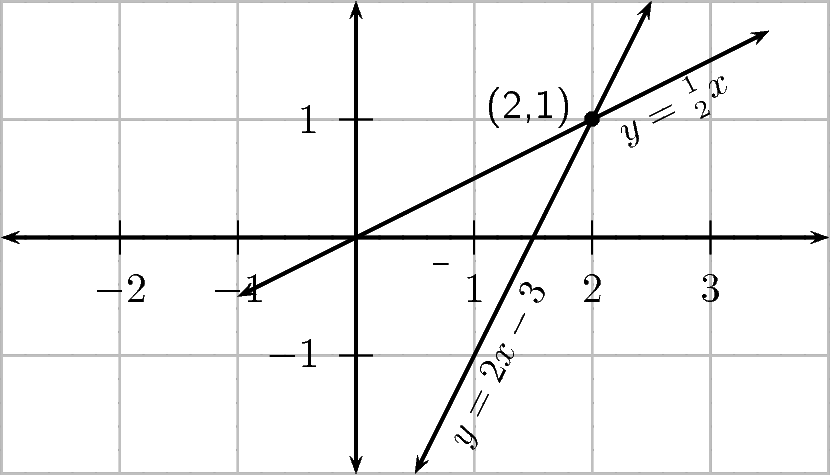
\includegraphics[width=.8\columnwidth]{col11306.imgs/m39257_MG10C10_006.png} % m39257;MG10C10\_006.png;;;6.0;8.5;
\begin{pspicture}(-3,-2)(4,2)
% \psgrid[gridcolor=lightgray,gridlabels=0,gridwidth=0.5pt]
\psaxes[dx=1,Dx=1,arrows=<->](0,0)(-3,-2)(4,2)
\pstextpath[c](-1.1,-0.3){\psplot[xunit=1,plotstyle=curve,arrows=<->]{0.5}{2.5}{x 2 mul 3 sub}}{\small{$y=2x-3$}}
\pstextpath[c](1.5,-0.3){\psplot[xunit=1,plotstyle=curve,arrows=<->]{-1}{3.5}{0.5 x mul}}{\small{$y=\frac{1}{2}x$}}
\uput[l](2,1.1){$(2,1)$}
\psdot(2,1)
\end{pspicture}

\vspace{2pt}
\vspace{.1in}
\rule[.1in]{\figurerulewidth}{.005in} \\
\end{center}
\end{figure}       
Die snypunt van die 2 grafieke is $(2;1)$. Dus, die oplossing van die stel gelyktydige vergelykings in $x=2$ en $y=1$.\par 
Dit kan ook algebraïes gevind word. \\
Stel die eerste vegelyking in die tweede vergelyking in:

\begin{equation*}
\begin{array}{ccl}\hfill x& =& 2y\hfill \\
 \hfill y& =& 2(2y)-3\hfill 
\end{array}
\end{equation*}
Los op vir $y$:
\begin{equation*}
\begin{array}{ccl}
 \hfill y-4y& =& -3\hfill \\
 \hfill -3y& =& -3\hfill \\ 
\hfill \therefore y& =& 1\hfill 
\end{array}
\end{equation*}
Stel die antwoord vir $y$ in die eerste vergelyking in:
\begin{equation*}
\begin{array}{ccl}
 \hfill x& =& 2(1)\hfill \\
 \therefore x&=& 2\hfill \end{array}
\end{equation*}

Let daarop dat beide metodes dieselfde oplossing gee.

\begin{wex}
{Gelyktydige vergelykings }
{Los die volgende stel gelyktydige vergelykings grafies op:
\begin{equation*}
\begin{array}{ccl}\hfill 4y+3x& =& 100\hfill \\ \hfill 4y-19x& =& 12\hfill \end{array}
\end{equation*}
}
{
\westep{Skryf albei vergelykings in die vorm $y=mx+c$}  

\begin{equation*}
\begin{array}{ccl}\hfill 4y+3x& =& 100\hfill \\
 \hfill 4y& =& 100-3x\hfill \\
 \hfill y& =& -\dfrac{3}{4}x + 25\hfill \end{array}
\end{equation*}
\\
\begin{equation*}
\begin{array}{ccl}\hfill 4y-19x& =& 12\hfill \\ \hfill 4y& =& 19x+12\hfill \\ \hfill y& =& \dfrac{19}{4}x+3\hfill \end{array}
\end{equation*}



\westep{Skets die grafieke van die 2 vergelykings op dieselfde assestelsel}
\setcounter{subfigure}{0}
\begin{figure}[H] % horizontal\label{m39257*id159679}
\begin{center}
\label{m39257*id159679!!!underscore!!!media}\label{m39257*id159679!!!underscore!!!printimage}
%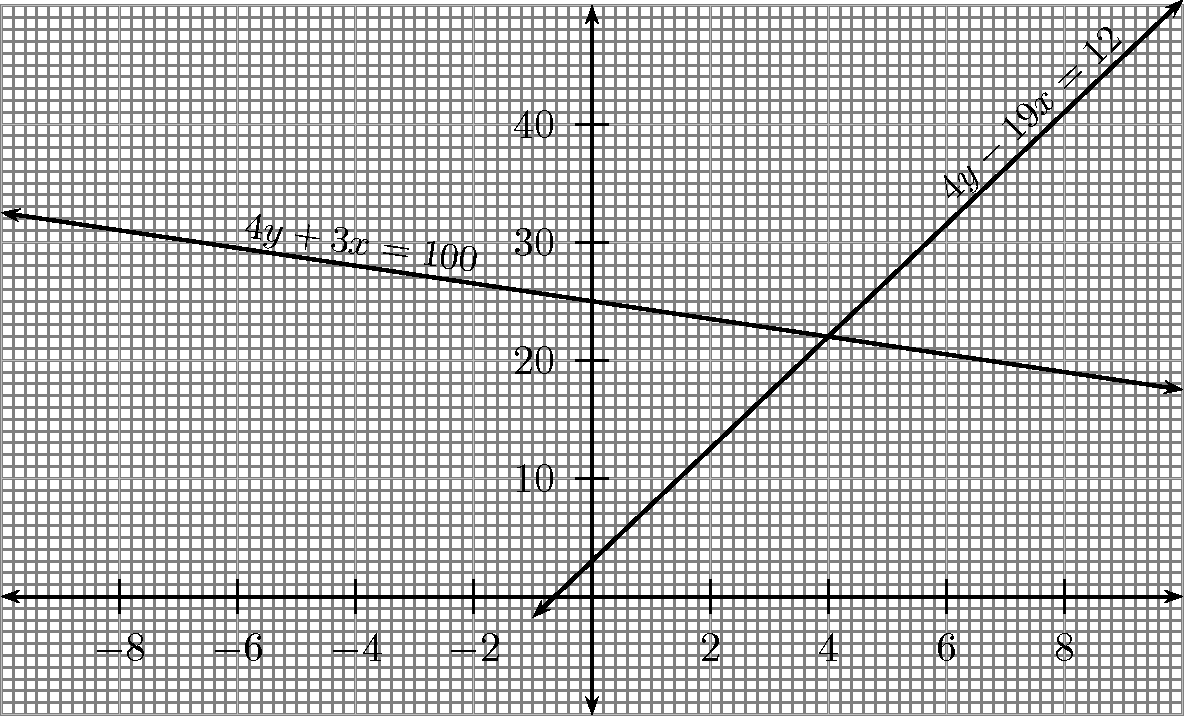
\includegraphics{col11306.imgs/m39257_MG10C10_007.png} % ;MG10C10\_007.png;;;6.0;8.5;
\begin{center}
\begin{pspicture}(-5,-1)(5,5)
%  \psgrid[subgriddiv=10,gridcolor=lightgray,gridlabels=0,gridwidth=0.1pt]
\psaxes[dx=1,dy=1,Dy=10,Dx=2,arrows=<->](0,0)(-5,-1)(5,5)
\pstextpath[c](-2,0.1){\psplot[xunit=0.5,yunit=0.1,plotstyle=curve,arrows=<->]{-10}{10}{0.75 x mul neg 25 add}}{\small{$4y+3x=100$}}
\pstextpath[c](2.2,0.1){\psplot[xunit=0.5,yunit=0.1,plotstyle=curve,arrows=<->]{-1}{10}{4.75 x mul 3 add}}{\small{$4y-19x=12$}}
\end{pspicture}
\end{center}

\vspace{2pt}
\vspace{.1in}
\end{center}
\end{figure}         

\westep{Vind die snypunt van die twee grafieke}
Die twee grafieke sny by $(4;22)$ 

\westep{Skryf die finale antwoord}
\begin{equation*}
\begin{array}{ccl}\hfill x& =& 4\hfill \\ \hfill y& =& 22\hfill \end{array}
\end{equation*}

}
\end{wex}

\begin{exercises}{}
{
 \Note{Om 'n stel gelyktydige vergelykings grafies op te los, in soms nie baie akkeuraat nie, maar dit is 'n waardevolle oplossings metode.}
\item Los algebraïes op: 
\begin{enumerate}[noitemsep, label=\textbf{\arabic*}. ] 
\item $3x-14y=0$ , $x-4y+1=0$
\item $x+y=8$, $3x + 2y = 21$
\item $y=2x+1$ , $x + 2y + 3 = 0$
\end{enumerate}

Los grafies op en bevestig jou oplossing algebraïes::

\begin{enumerate}[noitemsep, label=\textbf{\arabic*}. ] 
\setcounter{enumi}{3}
\item  $x+2y=1$, $\frac{x}{3} + \frac{y}{2} = 1$
\item $5= x+y$ , $-x = y-2$
\item $3x - 2y = 0$ , $x - 4y + 1 = 0$

\end{enumerate}


\par \raisebox{-5 pt}{
\includegraphics[width=0.5cm]{col11306.imgs/summary_www.png}} Kry die oplossing met die kortkodes:
\par \begin{tabular}[h]{cccccc}
(1.) lxq  &  (2.) lxl  &  (3.) lxi  &  (4.) lx3  & \end{tabular}
}
\end{exercises}

\section{Woordprobleme}

$ \hspace{-5pt}\begin{array}{cccccccccccc}   
\includegraphics[width=0.75cm]{col11306.imgs/summary_fullmarks.png} &   \end{array} $ \hspace{2 pt}\raisebox{-5 pt}{} {(section shortcode: MG10079 )} \par

Die doel van hierdie afdeling is om vir jou die vaardighede te leer om ’n probleem te neem en dit wiskundig te
formuleer sodat dit opgelos kan word.


\subsection*{Strategie vir die oplos van probleme}

\begin{enumerate}[noitemsep, label=\textbf{\arabic*}. ] 
\item Lees die HELE vraag!
\item Bepaal wat gevra word.
\item Gebruik (’n) veranderlike(s) om die onbekende getalle/hoeveelhede word voor te stel, $x$.
\item  Herskryf die inligting wat gegee is in terme van die veranderlike(s). Dus, vertaal die woorde in algebraïese
taal.
\item Stel ’n vergelyking of ’n stel gelyktydige vergelykings (’n Wiskundige model) op om die onbekende te kry.
\item Los die vergelyking algebraïes op om die oplossing te vind.
\item Toets die oplossing.
\end{enumerate}

\begin{wex}
{Oplos van woordprobleme}
{
 ’n Winkel verkoop tweewielfietse en driewiele. In totaal is daar $7$ fietse (fietse sluit tweewielfietse en driewiele in) en $19$ wiele. Bepaal hoeveel van elke soort fiets is daar.
}
{
\westep{Ken veranderlike toe aan die onbekende}
Laar $b$ die aantal tweewielfietse wees  \\
en laat $7-b$  die aantal driewiele wees: 

\westep{Stel 'n vergelyking op}
\begin{equation*}
\begin{array}{ccc}\hfill 2b+3(7-b)& =& 19\hfill \end{array}
\end{equation*}


\westep{Herrangskik en los po vir $b$}
\begin{equation*}
\begin{array}{ccl}
 \hfill 2b + 21 - 3b& =& 19\hfill \\
\hfill - b& =& -2\hfill \\
 \hfill \therefore b& =& 2\hfill 
\end{array}
\end{equation*}

\westep{Bereken die aantal driewiele}
\begin{equation*}
\begin{array}{ccl}
\\ \hfill  7 - 2 & =& 5\hfill \\
 \therefore \mbox{aantal driewiele}& =& 5
\end{array}
\end{equation*}

\westep{Skryf die finale antwoord}
 Daar is $5$ driewiele en $2$ fietse.

}       
\end{wex}

\begin{wex}{Oplos van die woordprobleme}{
Bongani en Jane is vriende. Bongani vat Jane se fisika toets en wil nie vr haar s\^e wat haar punt is nie. Hy weet sy hou nie baie van wiskunde nie en besluit om haar te terg. Bongani s\"e 
'ek het $2$ punte meer as jy en ons twee saam het $14$, hoeveel het ons elk gekry?'}
{
\westep{Ken veranderlikes toe aan die onbekendes}
Ons het twee onbekendes. Bongani se punt en Jane se punt 
\\Gestel Bongani het $t$ en Jane het $j$ punte. 

\westep{Stel 'n sisteem van vergelykings op}
\\Bongani het $2$ meer as Jane.
\begin{equation*}
t=j+2
\end{equation*}

Saam her hulle $14$ punte.

\begin{equation*}
t+j=14
\end{equation*}

\westep{Gebruik die eerste vergelyking om $t$ uit te druk in terme van $j$}
\begin{equation*}
t=j+2
\end{equation*}

\westep{Vervang in die tweede vergelyking in}
\begin{equation*}
    \begin{array}{ccc}\hfill t+j& =& 14\hfill \\
	\hfill (j+2)+j& =& 14\hfill \\

    \end{array}
\end{equation*}

\westep{Herrangskik en los op vir $j$}
\begin{equation*}
    \begin{array}{ccl}\hfill 2j& =& 14 - 2\hfill \\
	\hfill \therefore 2j& =& 12\hfill \\
\hfill \therefore j &=& 6 \hfill

    \end{array}
\end{equation*}

 \westep{Vervang die waarde van $j$ terug in die eerste vergelyking in los op vir $t$}
\begin{equation*}
\begin{array}{ccl}\hfill t& =& j+2\hfill \\ & =& 6+2\hfill \\ & =& 8\hfill \end{array}
\end{equation*}
\\
\westep{Kontroleer dat die oplossng beide oorspronklike vergelykings bevredig}
\westep{Skryf die finale antwoord}
Bongani het $8$ en Jane het  $6$ gekry.\\
}
\end{wex}

\begin{wex}
{Wiskundige modellering}
{
’n
Vrugteskommel kos R$~2,00$ meer as ’n sjokolade melkskommel. As $3$ vrugteskommels en $5$ sjokolade melkskommels saam  R$~78,00$, kos,
bepaal die afsonderlike pryse.}

{
\westep{Ken veranderlikes toe aan die onbekendes}  
Gestel die prys van ’n sjokelade melkskommel is $x$ 
\\ rand en die prys van ’n vrugteskommel is  $y$ rand.


\westep{Stel die sisteem van vergelykings op}
\begin{equation*}
\begin{array}{ccl} \hfill y &=& x+2 \hfill \\
\hfill 3y+5x& =& 78\hfill 
\end{array}
\end{equation*}

\westep{Vervang die eerste vergelyking in die tweede}
\begin{equation*}
\begin{array}{ccl}\hfill 3(x+2)+5x& =& 78\hfill \\
\end{array}
\end{equation*}

\westep{Herrangskik en los op vir $x$}
\begin{equation*}
\begin{array}{ccl}
 \hfill 3x+6+5x& =& 78\hfill \\ 
\hfill 8x& =& 72\hfill \\ 
\hfill \therefore x& =& 9\hfill \\  \end{array}
\end{equation*}

\westep{Vervang waarde van $x$ terug in die eerste vergelyking in en los op vir $y$}
\begin{equation*}
\begin{array}{ccl}
\hfill y& =& x+2\hfill \\
 \hfill & =& 9+2\hfill \\ 
\hfill & \therefore =& 11\hfill  \end{array}
\end{equation*}
\westep{Kontroleer dat die oplossing beide oorspronklike vergelykings bevredig}
\westep{Skryf die finale antwoord}
Een sjokelade melkskommel kos R$~9,00$ en een vrugteskommel
kos R$~ 11,00$.
}
\end{wex}

\begin{wex}
{Los woordprobleme op }
{
Die produk van twee opeen volgende negatiewe heelgetalle is $1122$. Vind die twee heelgetalle.
} 
{
\westep{Ken veranderlikes toe aan die onbekendes}
Gestel die eerste heelgetal is $n$ 
\\Dan is die tweede heelgetal $n+1$.\par 

\westep{Stel die vergelyking op}  
\begin{equation*}
\begin{array}{cll}\hfill n(n+1)& =& 1122\hfill \end{array}
\end{equation*}

\westep{Brei uit en los op vir $n$}
\begin{equation*}
    \begin{array}{cll}
	\hfill n^{2} + n =& 1122\hfill \\
\hfill n^{2} + n - 1122 =& 0\hfill \\
\hfill (n+34)(n-33) =& 0\hfill \\
	\hfill \therefore  n =& -34 \hfill \\
\hfill \mbox{ or } n =& 33\hfill 
    \end{array}
\end{equation*}

\westep{Integers must be negative}
\begin{equation*}
    \begin{array}{cll}
	\hfill \therefore n =& -34\hfill \\
\hfill n + 1 =& -34\ + 1 \hfill \\
\hfill  =& -33\hfill \\

    \end{array}
\end{equation*}

\westep{Skryf finale antwoord} 
Die twee opeenvolgende negatiewe heelgetalle is $-34$ e n$-33$.
}
\end{wex}

\begin{exercises}{Woordprobleme}
{
\begin{enumerate}[noitemsep, label=\textbf{\arabic*}. ] 
\item Twee vliegtuie vlieg na mekaar toe vanat lughauwens $1~200$ km van mekaar af. Een vlieg teen $250$ km/h en die ander teen $350$ km/h. As hulle dieselfde tyd vertrek, hoe lank sal dit hulle neem om by mekaar verby te vlieg?
\item Kadesh het $20$ hempde gekoop teen 'n totale bedrag van R$~980$. As die grrot hempde R$~50$ en die klieneres R$~40$, hoeveel van elke groote het hy gekoop?
\item Die diagonaal van ’n reghoek is $25~$cm meer as die wydte. Die lengte van die reghoek is $17~$cm meer as die wydte. Wat is die afmetings van die reghoek?  
\item Die som van $27$ en $12$ is $73$ meer as ’n onbekende getal. Vind die onbekende getal
\item Die twee kleiner hoeke van ’n reghoekige driehoek is in die verhouding $1:2$. Wat is die groottes van die
twee hoeke?
\item Die lengte van 'n reghoek is tweemaal die breedte. As die oppervlakke $128$ cm$^{2}$ is, bepaal die lengte en breedte.       
\item As $4$ keer ’n getal met $7$, vermeerder word, is die resultaat $15$ minder as die vierkant (kwadraat) van die
getal. Vind die getal wat hierdie stelling bevredig deur ’n vergelyking op te stel en dan op te los.
\item Die lengte van ’n reghoek is $2~$cm cm meer as die wydte van. Die omtrek van die reghoek is  $20~$cm. Vind die lengte en breedte van die reghoek.
\item Vian het $1~l$ liter van ’n mengsel wat $69\%$ out bevat. Hoeveel water moet Vian bygooi om die mengsel $50\%$ sout te maak? Skryf jou antwoord as ’n breukdeel van ’n liter.
       
\end{enumerate}

\par \raisebox{-5 pt}{
\includegraphics[width=0.5cm]{col11306.imgs/summary_www.png}} Kry die oplossing met die kortkodes:
\par \begin{tabular}[h]{cccccc}
(1.) lcy  &  (2.) lcV  &  (3.) lcp  &  (4.) lcw  &  (5.) lcd  &  (6.) lcf  &  (7.) lcv  & \end{tabular}
}
\end{exercises}

\section{Vergelykings met letterkoëffisiënte (Lettervergelykings)}
 $ \hspace{-5pt}\begin{array}{cccccccccccc}   
\includegraphics[width=0.75cm]{col11306.imgs/summary_fullmarks.png} &   \end{array} $ \hspace{2 pt}\raisebox{-5 pt}{} {(section shortcode: MG10078 )}\par
%   \label{m39258*eip-798}
%             \ssection{ Equations and inequalities: Literal equations}
%             \nopagebreak
%             

’n Vergelyking met letterkoëffisiënte is een wat verskeie letters of veranderlikes bevat. Voorbeelde sluit die area
van ’n sirkel ($A=\pi{r}^{2}$) in en die formule vir die berekening van spoed ($s=\frac{d}{t}$). In hierdie afdeling sal jy leer hoe om vergelykings met letterkoëffisiënte op te los in terme van een van die veranderlikes. Om dit te doen, sal jy die beginsels oor die oplos van vergelykings wat jy geleer het, gebruik en toepas om die woordvergelykings te herrangskik. Die oplos van vergelykings met letterkoëffisiënte staan ook bekend as verandering van die onderwerp van ’n formule.
 
Wanneer jy lettervergelykings oplos, behoort jy die volgende in gedagte te hou:
\begin{itemize}
\item Ons isoleer die onbekende deur te vra wat daaraan verbind is en hoe dit daaraan verbind is en dan doen
ons die teenoorgestelde bewerking (aan beide kante as ’n geheel).
\item As die onbekende veranderlike in twee of meer terme voorkom, haal ons dit uit as ’n gemeenskaplike faktor. 
\item  As ons weerskante die vierkantswortel moet neem, onthou dat daar ’n positiewe sowel as ’n negatiewe
antwoord mag wees.
\item  As die onbekende veranderlike in die noemer is, dan vind ons die kleinste gemene noemer (KGN), ver-
menigvuldig weerskante met die KGN en gaan dan voort om die probleem op te los.
\end{itemize}


\begin{wex}
{oplos van 'n lettervergelykings}
{
Die area van ’n driehoek is $A=\frac{1}{2}bh$. Wat is die hoogte van die driehoek in terme van die basis en area?
}
{
\westep{Isoleer die verlangde veranderlike}
Ons herrangskik die vergelyking sodat die $h$ aan die een kant
van die gelykaanteken is en die res van die veranderlikes aan die
ander kant van die gelykaanteken.
\begin{equation*}
    \begin{array}{cccc}\hfill A& =& \frac{1}{2}bh\hfill & \\
	\hfill 2A& =& bh\hfill & \hfill \\
	\hfill \frac{2A}{b}& =& h\hfill 
    \end{array}
\end{equation*}

\westep{Skryf die finale antwoord} 
Die hoogte van ’n driehoek word gegee deur: $h=\dfrac{2A}{b}$
} 
\end{wex}

\begin{wex}
{Oplos van lettervergelykings}
{
Gegee die formule $h=\dfrac{H}{R+r} \times R$, los op vir $R$.
}
{
\westep{Kry $R$ alleen aan die een kant van die vergelykings}
\begin{equation*}
    \begin{array}{ccll}\hfill h(R+r)& =& H \times R\hfill & \\
	\hfill hR + hr& =& HR\hfill & \hfill \\
	\hfill hr & =& HR - hR\hfill \\
\hfill hr& =& R(H - h)\hfill \vspace{5pt}\\ 
\hfill \therfore R & =& \dfrac{hr}{H-h}\hfill 
    \end{array}
\end{equation*}

\westep{Skryf die finale antwoord} 
$R = \dfrac{hr}{H-h}$
} 
\end{wex}


\begin{exercises}{}
{
\begin{enumerate}[noitemsep, label=\textbf{\arabic*}. ] 
\item Los op vir $t$: $v=u+at$
\item Los op vir $x$: $ax-bx=c$ \vspace{5pt}
\item Los op vir $x$: $\dfrac{1}{b}+\dfrac{2b}{x}=2$\vspace{5pt}
\item Los op vir $r$: $V = \pi r^{2} h$
\item Druk $l$ uit in terme van $b$ en $H$: $\sqrt{l^{2}+b^{2}}=H$
\item Los op vir $i$: $A=P(1+i)^{n}$
\item Los op vir $h$: $A=2\pi rh + 2 \pi r$
\item Los op vir $b$: $V=l \times b \times h$
\item Los op vir $h$: $V=\frac{1}{3}\pi r^{2}h$
\end{numerate}

\par \raisebox{-5 pt}{
\includegraphics[width=0.5cm]{col11306.imgs/summary_www.png}} Kry die antwoorde met die kort kodes:
\par \begin{tabular}[h]{cccccc}
(1.) lgw  &  (2.) lgw  &  (3.) lgw  & \end{tabular}
}
\end{exercises}

\section{Lineêre ongelykhede}
\nopagebreak
$ \hspace{-5pt}\begin{array}{cccccccccccc}   
\includegraphics[width=0.75cm]{col11306.imgs/summary_fullmarks.png} &   
\includegraphics[width=0.75cm]{col11306.imgs/summary_video.png} &   \end{array} $ \hspace{2 pt}\raisebox{-5 pt}{} {(section shortcode: MG10073 )} \par 


\begin{Aktiwiteit}{Line\^ere ongelykhede}
{
Stel die volgende voor op getallelyne en gebruik intervalnotasie:
\begin{enumerate}[noitemsep, label=\textbf{\arabic*}. ] 
\item $x<4$
\item $x\leq 4$
\item $x\geq 4$
\item $x>4$
\end{enumerate}
}
\end{activity}

’n Lineêre ongelykheid is soortgelyk aan ’n lineêre vergelyking aangesien die hoogste eksponent van die veranderlike $1$. is. Die volgende is voorbeelde van lineêre ongelykhede.\par 

\begin{equation*}
\begin{array}{ccc}\hfill 2x+2& \leq& 1\hfill \\ \hfill \dfrac{2-x}{3x+1}&\geq& 2\hfill \\ \hfill \frac{4}{3}x-6&<& 7x+2\hfill \end{array}
\end{equation*}
Die metodes wat gebruik word om lineêre ongelykhede op te los, is soortgelyk aan dié wat gebruik word om
lineêre vergelykings op te los. Die enigste verskil kom voor wanneer daar vermenigvuldiging met of deling
deur ’n negatiewe getal is. Ons weet byvoorbeeld dat
t $8>6$. As beide kante van die ongelykheid gedeel word (byvoorbeeld deur  $-2$ sien ons $-4 > -3$. Dus moet die ongelykheid omkeer, wat beteken
$-4<-3$.

\Tip{Wanneer beide kante van ’n ongelykheid met ’n negatiewe getal vermenigvuldig, of gedeel word, verander die rigting van
die ongelykheid. Om hierdie rede mag ons nie met ’n veranderlike vermenigvuldig as
ons nie weet nie wat die onbekende (veranderlike) se teken is nie.}

Byvoorbeeld, as  $x<1$, dan $-x>-1$.
Om ’n ongelykheid met behulp van 'n gewone gewone vergelyking op te los, sal ons eers die gewone vergelyking oplos. Los op $2x+2=1$.

\begin{equation*}
\begin{array}{ccl}\hfill 2x+2& =& 1\hfill \\ \hfill 2x& =& 1-2\hfill \\ \hfill 2x& =& -1\hfill \\ \hfill x& =& -\frac{1}{2}\hfill \end{array}
\end{equation*}
As ons hierdie antwoord op ’n getallelyn voorstel, kry ons:\par 

\setcounter{subfigure}{0}
\begin{figure}[H] % horizontal\label{m39254*id157630}
\begin{center}
\label{m39254*id157630!!!underscore!!!media}\label{m39254*id157630!!!underscore!!!printimage}
%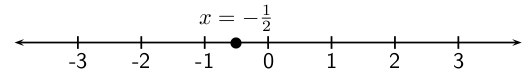
\includegraphics[width=.8\columnwidth]{col11306.imgs/m39254_MG10C10_001.png} % m39254;MG10C10\_001.png;;;6.0;8.5;
\begin{center}
\begin{pspicture}(-4,0.75)(4,1.75)
%\psgrid
\psline[arrows=<->](-4,1)(4,1)
\psdot[dotsize=5pt](-0.5,1)
\multido{\n=-3+1}{7}
{\uput[d](\n,1){$\n$}
\psline(\n,1.1)(\n,0.9)}
\uput[u](-0.5,1){$x=-\frac{1}{2}$}
\end{pspicture}
\end{center}
\vspace{2pt}
\vspace{.1in}
\end{center}
\end{figure}       
\par 
Kom ons los nou die ongelykheid $2x+2\leq1$ op.\par 


\begin{equation*}
\begin{array}{ccl}\hfill 2x+2& \leq& 1\hfill \\ \hfill 2x& \leq& 1-2\hfill \\ \hfill 2x& \leq& -1\hfill \\ \hfill x& \leq& -\frac{1}{2}\hfill \end{array}
\end{equation*}
As ons hierdie antwoord op ’n getallelyn voorstel, kry ons:\par 

\setcounter{subfigure}{0}
\begin{figure}[H] % horizontal\label{m39254*id157774}
\begin{center}
\label{m39254*id157774!!!underscore!!!media}\label{m39254*id157774!!!underscore!!!printimage}
%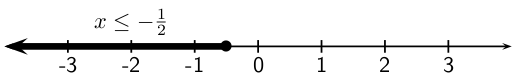
\includegraphics[width=.8\columnwidth]{col11306.imgs/m39254_MG10C10_002.png} % m39254;MG10C10\_002.png;;;6.0;8.5;
\begin{center}
\begin{pspicture}(-4,0.75)(4,1.75)
%\psgrid
\psline[arrows=<->](-4,1)(4,1)
\psdot[dotsize=5pt](-0.5,1)
\multido{\n=-3+1}{7}
{\uput[d](\n,1){$\n$}
\psline(\n,1.1)(\n,0.9)}
\uput[u](-2,1){$x\le-\frac{1}{2}$}
\psline[linewidth=3pt]{->}(-0.5,1)(-4,1)
\end{pspicture}
\end{center}
\vspace{2pt}
\vspace{.1in}
\end{center}
\end{figure}       
\par 

As ons hierdie oplossing in intervalnotasie uitdruk skryf ons $(-\infty ~;-\frac{1}{2}]$.\par
\Note{Aanvaar $x \in \mathbb{R}$ as die versamelling getalle nie gespesifiseer word nie. }
Soos jy kan sien, vir die vergelyking is daar slegs ’n enkele waarde van  $x$ waarvoor die vergelyking waar is. Vir
die ongelykheid is daar egter ’n hele versameling waardes waarvoor die ongelykheid waar is. Dit is die groot
verskil tussen gewone vergelykings (gelykhede) en ongelykhede.\par 

\setcounter{subfigure}{0}
\begin{figure}[H] % horizontal\label{m39254*inequalities-1}
\textnormal{Khan academy video on inequalities - 1}\vspace{.1in} \nopagebreak
\label{m39254*yt-media4}\label{m39254*yt-video4}
\raisebox{-5 pt}{ 
\includegraphics[width=0.5cm]{col11306.imgs/summary_www.png}} { (Video:  MG10074 )}
\vspace{2pt}
\vspace{.1in}
\end{figure}    

\setcounter{subfigure}{0}
\begin{figure}[H] % horizontal\label{m39254*inequalities-2}
\textnormal{Khan academy video on inequalities - 2}\vspace{.1in} \nopagebreak
\label{m39254*yt-media5}\label{m39254*yt-video5}
\raisebox{-5 pt}{ 
\includegraphics[width=0.5cm]{col11306.imgs/summary_www.png}} { (Video:  MG10075 )}
\vspace{2pt}
\vspace{.1in}
\end{figure}  
  
\begin{wex}
{Lineêre ongelykhede }
{
Los op vir $r$: $6-r>2$ \\
Stel jou antwoord voor op ’n getallelyn en in interval notasie.}
{ 
\westep{Herrangskik en los op vir $r$}  
\begin{equation*}
\begin{array}{ccl}\hfill -r&>&2-6\\ \hfill -r&>&-4\end{array}
\end{equation*}
\westep{Wanneer jy met ’n negatiewe getal vermenigvuldig, draai die rigting
van die ongelykheid om.}

\begin{equation*}
r<4
\end{equation*}


\westep{Stel die oplossing voor op ’n getallelyn.}

\setcounter{subfigure}{0}
\begin{figure}[H] % horizontal\label{m39254*id157937}
\begin{center}

%\includegraphics{col11306.imgs/m39254_MG10C10
% _003.png} % ;MG10C10\_003.png;;;6.0;8.5;
\begin{center}
\begin{pspicture}(-1,0.4)(6,1.6)
%\psgrid
\psline[arrows=<->](-1,1)(6,1)
\multido{\n=0+1}{6}
{\uput[d](\n,1){$\n$}
\psline(\n,1.1)(\n,0.9)}
\uput[u](2,1){$r<4$}
\psline[linewidth=3pt]{->}(4,1)(-1,1)
\psdot[dotsize=5pt,dotstyle=o](4,1)
\end{pspicture}
\end{center}
}
\vspace{2pt}
\vspace{.1in}
\end{center}
\end{figure}    

\westep{Druk die antwoord uit in intervalnotasie}
\begin{equation*}
(- \infty~;~4)   
\end{equation*}
}
\end{wex}

\begin{wex}{Los line\^ere ongelykhede op}
{
Los op vir $q$: $4q+3<2(q+3)$ \\
Stel die antwoord voor op 'n getallelyn en in intervalnotasie.
}
{
\westep{Brei die hakies uit}  
\begin{equation*}
\begin{array}{ccl}\hfill 4q+3& <& 2(q+3)\hfill \\ \hfill 4q+3& <& 2q+6\hfill \end{array}
\end{equation*}

\westep{Herrangskik en los op vir $q$}
\begin{equation*}
\begin{array}{ccl}\hfill 4q+3& <& 2q+6\hfill \\ \hfill 4q-2q& <& 6-3\hfill \\ \hfill 2q& <& 3\hfill \end{array}
\end{equation*}


\westep{Deel beide kante deur $2$}  
\begin{equation*}
\begin{array}{ccccc}\hfill 2q& <& 3\hfill &  \\ \hfill q& <& \frac{3}{2}\hfill & \end{array}
\end{equation*}

\westep{Stel die oplossing voor op ’n getallelyn} 

\setcounter{subfigure}{0}
\begin{figure}[H] % horizontal\label{m39254*id158287}
\begin{center}
\label{m39254*id158287!!!underscore!!!media}\label{m39254*id158287!!!underscore!!!printimage}
%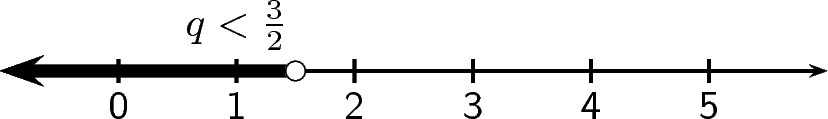
\includegraphics{col11306.imgs/m39254_MG10C10_004.png} % ;MG10C10\_004.png;;;6.0;8.5;
\begin{center}
\begin{pspicture}(-1,0.4)(6,1.6)
%\psgrid
\psline[arrows=<->](-1,1)(6,1)
\multido{\n=0+1}{6}
{\uput[d](\n,1){$\n$}
\psline(\n,1.1)(\n,0.9)}
\uput[u](1,1){$q<\frac{3}{2}$}
\psline[linewidth=3pt]{->}(1.5,1)(-1,1)
\psdot[dotsize=5pt,dotstyle=o](1.5,1)
\end{pspicture}
\end{center}

\vspace{2pt}
\vspace{.1in}
\end{center}
\end{figure}   

\westep{Druk die antwoord uit in itervalnotasie}
\begin{equation*}
(- \infty~;~\frac{3}{2})
\end{equation*}
}
\end{wex}


\begin{wex}
{Los saamgestelde line\^ere ongelykhede op }
{Los op vir $x$: $5\leq x+3<8$ \\
Stel die oplossing voor op 'n getallelyn en in intervalnotasie.}  
{
\westep{Trek $3$ af van alle terme}
\begin{equation*}
\begin{array}{cccll}\hfill 5-3 &\leq& x+3-3 &<& 8-3\hfill \\
		  \hfill 2&\leq& x &<&5 \hfill
\end{array}
\end{equation*}

\westep{Stel die oplossing voor op ’n getallelyn.}

\setcounter{subfigure}{0}
\begin{figure}[H] % horizontal\label{m39254*id158459}
\begin{center}
\label{m39254*id158459!!!underscore!!!media}\label{m39254*id158459!!!underscore!!!printimage}
%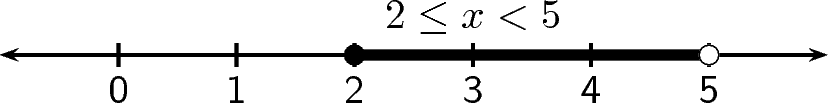
\includegraphics{col11306.imgs/m39254_MG10C10_005.png} % ;MG10C10\_005.png;;;6.0;8.5;
\begin{center}
\begin{pspicture}(-1,0.4)(6,1.6)
%\psgrid
\psline[arrows=<->](-1,1)(6,1)
\multido{\n=0+1}{6}
{\uput[d](\n,1){$\n$}
\psline(\n,1.1)(\n,0.9)}
\uput[u](3,1){$2\le x < 5$}
\psline[linewidth=2.5pt](2,1)(5,1)
\psdot[dotsize=5pt,dotstyle=o](5,1)
\psdot[dotsize=5pt](2,1)
\end{pspicture}
\end{center}

\vspace{2pt}
\vspace{.1in}
\end{center}
\end{figure}       
}

\westep{Druk antwoord uit in intervalnotasie}
\begin{equation*}
[~2~;~5)
\end{equation*}
\end{wex}


\begin{exercises}{ }
{
Los op vir $x$ en stel die antwoord voor op 'n getallelyn en in intervalnotasie:
\begin{enumerate}[noitemsep, label=\textbf{\arabic*}. ] 

    \item $3x+4>5x+8$
    \item $3(x-1)-2\leq 6x+4$ \vspace{5pt}
    \item $\dfrac{x-7}{3}>\dfrac{2x-3}{2}$\vspace{5pt}
    \item $-4(x-1)<x+2$\vspace{5pt}
    \item $\dfrac{1}{2}x+\dfrac{1}{3}(x-1)\geq \dfrac{5}{6}x-\dfrac{1}{3}$ \vspace{5pt}
    \item $-2\leq x-1<3$ 
    \item $-5<2x-3\leq7$ 
\item $7(3x+2)-5(2x-3)>7$
    \end{enumerate}


\par \raisebox{-5 pt}{
\includegraphics[width=0.5cm]{col11306.imgs/summary_www.png}} Find the answers with the shortcodes:
\par \begin{tabular}[h]{cccccc}
(1.) lcJ  &  (2.) lcS  &  (3.) lch  & \end{tabular}
}
\end{exercises}

\Opsomming
\nopagebreak
\label{m39263} $ \hspace{-5pt}\begin{array}{cccccccccccc}   \end{array} $ \hspace{2 pt}\raisebox{-5 pt}{
\includegraphics[width=0.5cm]{col11306.imgs/summary_www.png}} {(section shortcode: MG10080 )} \par 

\begin{itemize}[noitemsep]
\item ’n Lineêre vergelyking is ’n vergelyking waar die hoogste mag van die veranderlike $1$. is. ’n Lineêre vergelyking het op die meeste een oplossing.
\item ’n Kwadratiese vergelyking is ’n vergelyking waar die hoogste mag van die veranderlike $2$. is. ’n Kwadratiese
vergelyking het op die meeste 2 oplossings
\item ’n Lineêre ongelykheid is soorgelyk aan ’n lineêre vergelyking en met die hoogste mag van die veranderlike
gelyk aan $1$.
\item Wanneer jy weerskante van ’n ongelykheid deel of vermenigvuldig met ’n negatiewe getal,
draai die rigting van die ongelykheid om. 
\item Wanneer 2 onbekende veranderlikes opgelos moet word, moet jy 2 vergelyking gebruik en hierdie vergelykings staan bekend as gelyktydige vergelykings. Daar is twee maniere waarop jy gelyktydige lineêre
vergelykings kan oplos: grafies en algebraïes om die vergelykings grafies op te los, trek jy ’n grafiek
van elke vergelyking en die oplossing sal die koördinate van die snypunt van die grafieke wees. Om die
oplossing algebraïes te vind, los jy een vergelyking op vir een veranderlike en stel dan daardie oplossing
in die ander vergelyking in om die tweede veranderlike se waarde te vind.
\item Lettervergelykings is vergelykings waar jy verskeie letters (veranderlikes) het en jy herrangskik die vergelyking om die oplossing te vind in terme van een van die letters (veranderlikes)
\item Wiskundige modellering is waar ons ’n vergelyking of ’n stel vergelykings opstel om ’n probleem wiskundig
voor te stel. Die oplossing van die vergelykings gee dan die oplossing van die probleem.
\end{itemize}

\begin{eocexercises}{}
{
 Los op:
\begin{enumerate}[noitemsep, label=\textbf{\arabic*}. ] 
\begin{multicols}{2} 
\item $2(p-1) = 3(p+2)$
\item $3-6k = 2k-1$
\item $m + 6(-m+1) + 5m = 0$
\item $2k + 3 = 2-3(k+3)$
\item $5t-1=t^{2}-(t+2)(t-2)$\vspace{5pt}
\item $3+\dfrac{q}{5} = \dfrac{q}{2}$ \vspace{5pt}
\item $5-\dfrac{2(m+4)}{m} = \dfrac{7}{m}$\vspace{5pt}
\item $\dfrac{2}{t} - 2 - \dfrac{1}{2} = \dfrac{1}{2}(1+\dfrac{2}{t})$\vspace{5pt}
\item $x^{2} - 3x + 2=0$
\item $y^{2} + y = 6$
\item $0=2x^{2} - 5x - 18$\vspace{5pt}
\item $(d+4)(d-3)-d=(3d-2)^{2} - 8d(d-1)$\vspace{5pt}
\item $5x+2\leq4(2x-1)$\vspace{5pt}
\item $\dfrac{4x-2}{6} > 2x+1$\vspace{5pt}
\item $\dfrac{x}{3} - 14 > 14 - \dfrac{x}{7}$\vspace{5pt}
\item $\dfrac{1-a}{2} - \dfrac{2-a}{3} \geq 1$\vspace{5pt}
\item $-5 \leq 2k + 1 < 5$\vspace{5pt}
\item $x-1=\dfrac{42}{x}$  
\end{multicols}
\end{enumerate}

Los die volgende lettervergelykings op:
\begin{enumerate}[noitemsep, label=\textbf{\arabic*}. ] 
\setcounter{enumi}{18}
\item Los op vir$i$: $P = VI$
\item Los op vir $m$: $E=mc^{2}$
\item Los op vir $t$: $v = u + at$\vspace{5pt}
\item Los op vir $f$: $\dfrac{1}{u} + \dfrac{1}{v} = \dfrac{1}{f}$\vspace{5pt}
\item Los op vir $C$: $F=\frac{9}{5}C + 32$\vspace{5pt}
\item Los op vir $y$: $m = \dfrac{y-c}{x}$\vspace{5pt}
\end{enumerate}

Los die volgende stelsels gelyktydige vergelykings op:
\begin{enumerate}[noitemsep, label=\textbf{\arabic*}. ] 
\setcounter{enumi}{24}
\item $7x+3y=13$ en $2x-3y=-4$  
\item $10=2x+y$ en $y=x-2$
\item $7x-41=3y$ en $17=3x-y$
\item $2y=x+8$ en $4y=2x-44$
\end{enumerate}

Vind die oplossings van die volgende probleme:
\begin{enumerate}[noitemsep, label=\textbf{\arabic*}. ] 
\setcounter{enumi}{28}
\item $\frac{7}{8}$ van ’n getal is $5$  meer as ’n derde van die getal. Vind die getal.
\item Drie liniale en twee penne kos saam R $21,00$. Een liniaal en een pen kos saam R $8,00$. Hoeveel kos ’n pen op sy eie en hoeveel kos ’n liniaal op
sy eie? 
\item ’n Man hardloop na ’n telefoon en terug in $15$ minute. Sy spoed na die telefoon is $5$ km/h en sy spoed terug is $4$ km/h. Wat is die afstand na die foon?.
\item Zanele en Piet rolskaats na mekaar toe op 'n reguit pad. Hulle begin $20$ km van mekaar af. Zanele skaars teen $15$ km/h en Piet teen $10$ km/h. Hoe ver sal Piet skaats voor dat hulle by mekaar uitkom?
\item As die prys van sjokelade met R $10$ verhoog word, kan ons $5$ minder sjokelades koop vir R $300$. Wat was die prys van elke sjokelade voor die prys verhoog het?
   
\end{enumerate}
\end{enumerate}

\par \raisebox{-5 pt}{
\includegraphics[width=0.5cm]{col11306.imgs/summary_www.png}} Vind die kortkodes met:
\par \begin{tabular}[h]{cccccc}
(1.) lcG  &  (2.) lc7  &  (3.) lcA  &  (4.) lco  &  (5.) lcs  &  (6.) lcH  &  (7.) lc6  &  (8.) lcF  &  (9.) lcL  &  (10.) lcM  & \end{tabular}
}
\end{eocexercises}